\documentclass[11pt]{beamer}
\usetheme{Antibes}
\usepackage[utf8]{inputenc}
\usepackage{amsmath}
\usepackage{amsfonts}
\usepackage{amssymb}
\usepackage{listings}
\usepackage[backend=bibtex]{biblatex} 
\graphicspath{{images/}}
%\author{}
%\title{}
%\setbeamercovered{transparent} 
%\setbeamertemplate{navigation symbols}{} 
%\logo{} 
%\institute{} 
%\date{} 
\subject{GPU Architecture} 
\addbibresource{HMM.bib}
\begin{document}

\begin{frame}
\title{HMM Inference with CUDA}
\subtitle{Marc Haubenstock \& Christian Brändle}

\titlepage
\end{frame}

%\begin{frame}
%\tableofcontents
%\end{frame}

\begin{frame}{Introduction}

A \emph{Hidden Markov Model} describe a \textbf{two-state stochastic process}.
There is a stochastic process that is stationary (which means its probabilistic features don't change over time) and a state space that is finite.

\end{frame}

\begin{frame}{Introduction cont.}
% figure for state transition table as finite state automaton
\begin{table}[h]
	\begin{center}
		\begin{tabular}{| c | c |}
			\hline
			\multicolumn{2}{|l|}{
				\begin{tabular}{ l }
					\emph{Finite state automatons} \\
				\end{tabular}
			} \\
			\hline
			& \\
			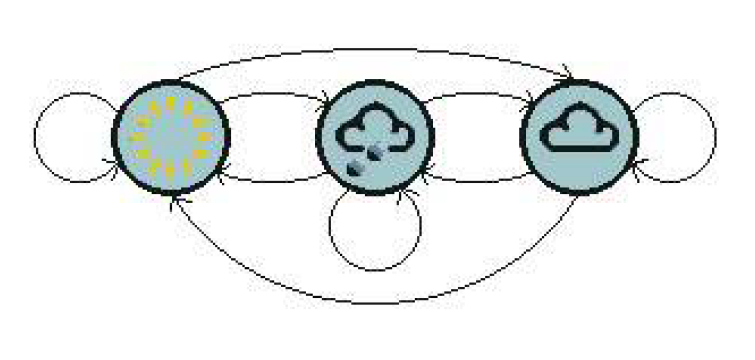
\includegraphics[width=0.25\textwidth]{./Images/FiniteStateAutomaton_1.png} & 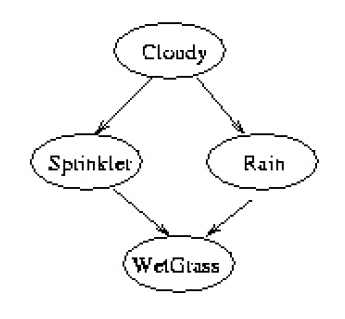
\includegraphics[width=0.25\textwidth]{./Images/FiniteStateAutomaton_2.png} \\
			\hline
			weather HMM \footcite{hmm_fb} & grass HMM \footcite{gm_bn} \\
			\hline
		\end{tabular}
	\end{center}
	\caption{Two finite state automatons that describe the state space of two different HMMs. Nodes correspond to states and edges to transition probabilites betwenn states that are bigger than $0$.}
	\label{tab:FiniteSA}
\end{table}


\end{frame}

\begin{frame}{Introduction cont.}
The important thing is that \textbf{the behaviour of the process given at time $t$ only depends on the immediate predecessor state}.

So the \emph{Markov property} states:

\begin{equation}
	P(S_t | S_1,S_2, \ldots S_{t-1}) = P(S_t | S_{t-1})
\end{equation}
\end{frame}

\begin{frame}{Introduction cont.}
Visually this can be shown with a graph model of a HMM as a sequence of hidden states $X_i$ and the corresponding obervations $Y_i$ - see figure \ref{fig:GraphModel}.

% GraphModelHMM_1.png
\begin{figure}[H]
	\centering
	
	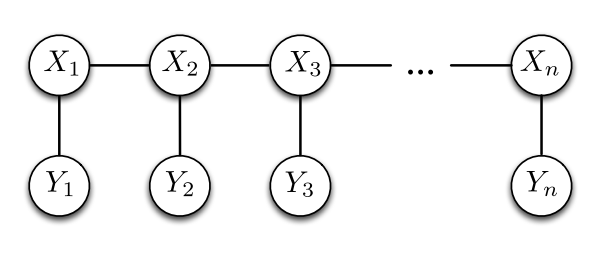
\includegraphics[width=0.66\textwidth]{./Images/GraphModelHMM_1.png}
	\caption{ \cite{hmm_II}}
	\label{fig:GraphModel}
\end{figure}

\end{frame}

\begin{frame}{Introduction cont.}
Furthermore, the corresponding \textbf{probability distribution only depend on the current state}. This is called the \emph{output independence assumption}.

\begin{equation}
P(O_t | O_1,O_2, \ldots O_{t-1}) = P(O_t | S_{t-1})
\end{equation}

The model itself is 'hidden' because we only can observe the outputs generated, namely the \emph{observation sequence} $O_1, O_2, \ldots,  O_T$.
\end{frame}

\begin{frame}{Introduction cont.}
\begin{figure}
\includegraphics[scale=0.25]{"symbols"}
\end{figure}
\end{frame}

\begin{frame}{Algorithms}
\begin{figure}[H]

\centering
\includegraphics[scale=0.4]{"FW"}
 \caption{Pesudo-Code for the Forward Algorithm \cite{cuhmm}}

\end{figure}

\end{frame}

\begin{frame}{Algorithms}
\begin{figure}[H]

\centering
\includegraphics[scale=0.4]{"vit"}
 \caption{Pesudo-Code for the Viterbi Algorithm \cite{cuhmm}}

\end{figure}
\end{frame}

\begin{frame}{Algorithms}
\begin{figure}[H]

\centering
\includegraphics[scale=0.3]{"BW"}
 \caption{Pesudo-Code for the Backward Forward Algorithm \cite{cuhmm}}

\end{figure}
\end{frame}

\begin{frame}{Algorithms}
\begin{figure}[H]

\centering
\includegraphics[scale=0.4]{"estimation"}
 \caption{Estimation of the A and B Matricies \cite{cuhmm}}

\end{figure}

The estimated values of the emission matrix B is not dependent on \(\epsilon(j)\), but should be on \(\gamma\), as it is defined in literature \cite{hmm}. 
\end{frame}

\begin{frame}{Implementation}
\begin{figure}[H]
\centering

\includegraphics[scale=0.2]{"3d_trellis"}
  \caption{Graphical representation of the data structure presented in \textit{A Cuda Implementation of Hidden Markov Models}\cite{cuhmm}}
\end{figure}
\end{frame}

\begin{frame}{Implementation cont.}
\begin{center}

\( D_{ij} = B_{O_i} .* C_i \times A_j \)

\end{center}

Where \( B_{O_i}\) is the row of the emission matrix at observation \(O_i\), \(C_i\) is the previous slice and \(A_j\) is the j\textsuperscript{th} column of the transition. matrix A.
\end{frame}

\begin{frame}{Implementation cont.}
\begin{figure}[H]
\centering

\includegraphics[scale=0.2]{"slice"}
  \caption{The computation of a slice\cite{cuhmm}}
\end{figure}
\end{frame}

\begin{frame}{Implementation cont.}
Finally a stipulation of the outlined method is that:

\begin{itemize}
\item The number of states and sequences must be a multiple of block size 16
\item The number of output sequences must be of the same length.
\end{itemize}
\end{frame}

\begin{frame}[fragile]{Forward}
\begin{verbatim}
__global__ initTrellis<<<M,N>>>(..){
  int obs_index = blockIdx.x * T_noOfObservations;
  int obs_start = dev_O_obsSequences_2D[obs_index];
  int idx_b_i_idxOs = threadIdx.x*V_noOfObsSymbols 
    + obs_start;
  int idx_alpha_0i = blockIdx.x * N_noOfStates 
    + threadIdx.x;
  int idx_pi_i = threadIdx.x;

  double alpha_0_i 
    = dev_Pi_startProbs_1D[idx_pi_i] * 
      dev_B[idx_b_i_idxOs];
  dev_3D_Trellis[idx_alpha_0i] = alpha_0_i;
}
\end{verbatim}
\end{frame}

\begin{frame}[fragile]{Forward}
\begin{verbatim}
// Computes the B matrix in term D = B .* C x A
ComputeBDevice << < M, N >> >
(M, V, T, N, 
dev_O_obsSequence_2D, dev_B_obsEmissionProbs_2D, i, dev_B);

// All dimensions are multipe of Warp Sizes
// Compute W =  B .* C
pointwiseMatrixMul << <M, N >> >(dev_W, dev_B,
&dev_3D_Trellis[(i - 1) * M * N]);

// Compute D = W x A
cublasMultiplyDouble(M, N_noOfStates, N, dev_W, 
dev_A_stateTransProbs_2D, &dev_3D_Trellis[i * M * N]);
\end{verbatim}
\end{frame}

\begin{frame}[fragile]{Forward}
\begin{verbatim}
for (int i = 0; i < M_noOfObsSequences; i++)
{
  int smBytes = 64 * sizeof(double);
  int grid = N_noOfStates / 64;
  reduce_1 <<< grid, 64, smBytes >>>
  (&last_slice[i*N_noOfStates], dev_A_odata);

  memcpyVector(..);

  host_likelihoods_1D[i] = host_A_odata[0] + 
    host_A_odata[1];

}
\end{verbatim}
\end{frame}


\begin{frame}[fragile]{Forward}
\begin{verbatim}
// FROM: NVIDIA Optimizing Parallel Reduction in CUDA
__global__ void reduc1(double* g_idata, double* g_odata){
  extern __shared__ double sdata[];
  int tid = threadIdx.x;
  int i = blockIdx.x*blockDim.x + threadIdx.x;
  sdata[tid] = g_idata[i];
  __syncthreads();
  for (int s = 1; s < blockDim.x; s *= 2){
    if (tid % (2 * s) == 0)
    {sdata[tid] += sdata[tid + s];}
    __syncthreads();
  }
  if (tid == 0){
    g_odata[blockIdx.x] = sdata[0];
\end{verbatim}
\end{frame}

%%%% VITERBI %%%%%%
\begin{frame}[fragile]{Viterbi - viterbi1D central algorithm}
\begin{verbatim}	
double p = a_ji * b_it;
double alpha_tm1j = 
dev_Alpha_trelis_2D[idx_alpha_tm1j];
double alpha_ti = 
dev_Alpha_trelis_2D[idx_alpha_ti];
double partPathProb_tm1j = alpha_tm1j * p;
if (partPathProb_tm1j >alpha_ti)
{
  dev_Alpha_trelis_2D[idx_alpha_ti] = 
  partPathProb_tm1j;
  // backpointers(t,i) = j
  dev_Gamma_trellis_backtrace_2D[idx_alpha_ti] = 
  idx_j;
}	
\end{verbatim}
\end{frame}

\begin{frame}[fragile]{Viterbi - kernel 1D - slicing}
\begin{verbatim}
int idx_m = blockIdx.x * blockDim.x + threadIdx.x;
// check if idx_m is out of range 
if (idx_m > M_noOfObsSequences)
  return;
  
// slice matrices according to idx_m
double *dev_Alpha_trelis_TN_2D = ...;
int *dev_Gamma_trellis_backtrace_TN_2D = ...
int* dev_O_obsSequence_1D = ...
int* dev_likeliestStateIndexSequence_1D = ...
\end{verbatim}
\end{frame}

\begin{frame}[fragile]{Viterbi - kernel 1D - tracking}
	\begin{verbatim}
// device memory initialization
TrellisInitialization2D(...);

// creating indices for viterbi1D
for (int idx_t = 1; idx_t < T; idx_t++)
  for (int idx_i = 0; idx_i < N; idx_i++)
    for (int idx_j = 0; idx_j < N; idx_j++)
    {
      viterbi1D(...);
    }
  // rescaling of Trellis'
  TrellisScaling2D(dev_Alpha_trelis_TN_2D, ...);

\end{verbatim}
\end{frame}

\begin{frame}[fragile]{Viterbi - kernel 1D - backtrack}
\begin{verbatim}
// extract most likely path of states 
// that generates observation
double partPathProb_optT = 0;
unsigned int idx_j = 0;
for (int idx_i = 0; idx_i < N; idx_i++) 
  if (idx_i == 0 || 
    dev_Alpha_trelis_TN_2D[(T - 1)*
    N + idx_i] > partPathProb_optT)
  {
    partPathProb_optT = 
      dev_Alpha_trelis_TN_2D[(T - 1)*
      N + idx_i];
    idx_j = idx_i;
  }

\end{verbatim}
\end{frame}

\begin{frame}[fragile]{Viterbi - kernel 1D - backtrack II}
\begin{verbatim}
dev_likeliestStates_1D[T - 1] = idx_j;
for (int idx_i = 1; idx_i < T; idx_i++)
{
  dev_likeliestStates_1D[T - 1 - idx_i] =
    dev_Gamma_trellis_backtrace_TN_2D[(T - idx_i)*
    N_noOfStates +
    dev_likeliestStates_1D[T - idx_i]];
}
\end{verbatim}
\end{frame}

\begin{frame}[fragile]{Baum-Welch}
\begin{verbatim}
for (int t = T_noOfObservations - 1; t >= 0; t--) {
 UpdateGammaGPU << <M, N >> >(..);
 UpdateEpsilonReductionErrorGPU <<<M, N >>>(..);
 if (t > 0){
  // Computes the B matrix in term D = B .* C x A
  // All dimensions are multipe of Warp Sizes
  // Compute W =  B .* C i.e. beta(t,i) * b_it
  ..
  for (int j = 0; j < N_noOfStates; j++){
   UpdateEpsilonGPU <<<M,N>>>
   (dev_epsilon_3D,dev_beta_3D,
    dev_3D_Trellis_Alpha,t,dev_likelihood,j,dev_D);
  } // end of for j
 } // end of if
} // end of for t
\end{verbatim}
\end{frame}

\begin{frame}[fragile]{Baum-Welch}
\begin{verbatim}
for (int t = T_noOfObservations - 1; t >= 0; t--) {
UpdateGammaGPU << <M, N >> >(..);
UpdateEpsilonReductionErrorGPU <<<M, N >>>(..);
 if (t > 0){
  // Computes the B matrix in term D = B .* C x A
  // All dimensions are multipe of Warp Sizes
  // Compute W =  B .* C i.e. beta(t,i) * b_it
  ..
  for (int j = 0; j < N_noOfStates; j++){
   UpdateEpsilonGPU <<<M,N>>>
   (dev_epsilon_3D, dev_beta_3D,
   dev_3D_Trellis_Alpha,t,dev_likelihood,j,dev_D);
  } // end of for j
 } // end of if
} // end of for t
\end{verbatim}
\end{frame}

\begin{frame}[fragile]{Baum-Welch}
\begin{verbatim}
ColumReduction_Height <<<1, N >>>
(epsilon_reduction_grid_error, M);
ColumReduction_Height <<<N,N>>>(dev_epsilon_3D, M);

ColumReduction_Height <<< N,V>>>
(dev_gamma_3D, M_noOfObsSequences);
ColumReductionGamma_Depth <<<1, N >>>
(dev_gamma_3D, 0, V,M, gamma_reduction_grid);

EstimateA <<<N, N>>>(..);

EstimateB <<<V, N>>>(..);
\end{verbatim}
\end{frame}

\begin{frame}{Evaluation}

 First we produce the transition and emission matrices $A$ and $B$. 
 Once the matrices have been generated we use the sequence generator of Liu to produce observation sequences of length $L = 16$. Both of these stages are performed on the CPU with regular C++ code.

\end{frame}

\begin{frame}[fragile]{Evaluation}

\begin{verbatim}
startBenchmark(..);
for (int i = 0; i < ITERATIONS; i++)
{
  // run kernel
}
stopBenchmark(..);
\end{verbatim}
Where \textit{startBenchmark} and \textit{stopBenchmark} are wrapper functions for \textit{cudaEventRecord}.

\end{frame}

\begin{frame}{Evaluation}
\begin{figure}[H]
\centering
\begin{tabular}{|l|l|}
\hline
GPU &GForce GTX 860M \\ \hline
CPU & intel i7-4710HQ @2.50 GHz with 8 GB of RAM  \\ \hline
OS & Windows 10 \\ \hline
CUDA & CUDA 7.5 CM 3.0 \\ \hline
Host Compiler & Visual Studio 2013 \\ \hline

\end{tabular}

\caption{Test Environment}
\end{figure}
\end{frame}

\begin{frame}{Evaluation}
\begin{figure}[H]
\centering
\begin{tabular}{|l|l|l|l|}
\hline
Data size (N $\times$ M) & Liu CPU & Liu GPU & GPU (Average of 1000)\\ \hline
64 $\times$ 64 & 687.7 & 10.2 & 13.6 \\ \hline
128 $\times$ 128 & 5621.9 & 19.74 & 18.15 \\ \hline
192 $\times$ 192 & 18990.5 & 40.93 & 35.93 \\ \hline
256 $\times$ 256 & 45031.6 & 71.77 & 47.20 \\ \hline
320 $\times$ 320 & 88090.8 & 128.44 & 77.09 \\ \hline
448 $\times$ 448 & 152374.8 & 208.08 & 124.99 \\ \hline
512 $\times$ 512 & 360899.3 & 410.17 & - \\ \hline

\end{tabular}

\caption{Comparing the run time of the forward algorithm in ms}
\end{figure}
\end{frame}

\begin{frame}{Evaluation}
\begin{figure}[H]
\centering
\begin{tabular}{|l|l|l|}
\hline
Data size (N $\times$ M) & CPU 1D & GPU 1D \\ \hline
64 $\times$ 64 & 208.53 & 902.71 \\ \hline

\end{tabular}

\caption{Comparing the run time of the Viterbi algorithm in ms}
\end{figure}
\end{frame}

\begin{frame}
\begin{figure}[H]
\centering
\begin{tabular}{|l|l|l|l|}
\hline
Data size (N $\times$ M) & Liu CPU & Liu GPU &GPU+CPU(Avg. of 1k)\\ \hline
64 $\times$ 64 & 2138.4 & 35.9 & 115.43 \\ \hline
128 $\times$ 128 & 7891.1.9 & 142.6 & 297.26 \\ \hline
192 $\times$ 192 & 57681.3 & 339.1 & 722.38 \\ \hline
256 $\times$ 256 & 136694.2 & 903.3 & - \\ \hline
320 $\times$ 320 & 267038.8 & 1328.6 & - \\ \hline
448 $\times$ 448 & 461297.6 & 2479.6 & - \\ \hline
512 $\times$ 512 & 1094036.4 & 6054.8 & - \\ \hline

\end{tabular}

\caption{Comparing the run time of the BW algorithm in ms}
\end{figure}
\end{frame}

\begin{frame}{Conclusion}
In general it can be seen that by using the GPU considerable performance gains can be made when applied to Hidden Markov Models. Further improvements can be made by using \textit{Texture Memory} \cite{cuhmm} as data structures such as the transition and emission matrices are read only for the forward and viterbi algorithm. Furthermore, \textit{dynamic parallelism} can be use to optimize the code further, as reductions can be spawned form inside CUDA kernels and thus don't require context switching back to the CPU. These could be topics for future projects.

\end{frame}



\end{document}